\chapter{Discussion and Conclusion}
\label{discuss} % Always give a unique label

The system has separate wheatstone bridges for each direction, giving ability to measure each component of the force independently. 

	Force-sensing devices were designed to fit daVinci cannula and sterile adapter and compensate tolerances by adjustment of set screws.
	
	Temperature dependence is not appropriate to do, since we have big systematic errors. First priority will be remove systematic errors.

Figure \ref{fig:Syst_err} shows X-component of the force measured with created device and using load cell. SNR of the system is high  it can be assumed that fluctuations in the output signal are due to systematic errors. 

For Z-direction device we got wide range of forces, because we cannot get high electronic gain, since the sensor is unbalanced caused by mechanical preloading of the sensor plate.


	Both devices should undergo sterilization. One of the devices goes inside the patient, meaning that it should be created using biocompatible materials. Current version of the device is not biocompatible. We can achieve biocompatibilty by using Stainless Steel as a device material and biocompatible epoxy to cover strain gauges, also teflon coated wires should be used for all electrical connections. Use of stainless steel will require change of the device dimensions, since the material has different elasticity. Also, epoxy cover can alter readings results.
	
	The real-time haptic feedback requires minimum data acquisition speed to be 1 kHz \cite{seungmoon_choi_effect_2004}. However, the current maximum speed is 588 Hz due to limitation of data transfers speed using serial communication with computer (115.2 Kbps). In order to increase the speed, we can change the communication channel to SPI (up to 10 Mbps) \cite{_uart_porotocol} or one of the wireless protocols, such as Bluetooth (up tp 1 Mbps) or wifi (up to 100 Mbps) \cite{_wireless_protocols}. Also, communication protocol between microcontroller and ADC can be changed from SPI to faster parallel communication. Additionally, the microcontroller can be changed to faster one, so it can support wireless communication. All these changes require change of the PCB design and microcontroller software. Also, in the PCB the amount of Wheatstone bridges and ADCs should be increased from 2 to 4 to reduce the overall size of the system by removing second PCB and master-slave communication.
	
	The designed devices measure forces in slightly higher than $\pm 11 N$ range. When the applied force exceeds the specified range, the device readings can be used to trigger safety alert.
	
	The required resolution should be at least 0.3 N and have error less than 0.05 N \cite{mack_interactive_2012}.
	
	Comparison of two Z-component of the force measurement methods have shown, that Z Device has lower 
	
We tried to measure force in Z-direction, but unfortunately results shown that developed system was not accurate and sensitive enough. To improve system we can suggest to change strain gauges to more sensitive ones. Since we have small room for deformation - around 0.3 mm, we can not afford more deformation by using thinner or longer plates. Therefore, we decided to use motor current readings for z-directional reading of the force.
	

\begin{figure}[h]
	\begin{center}
	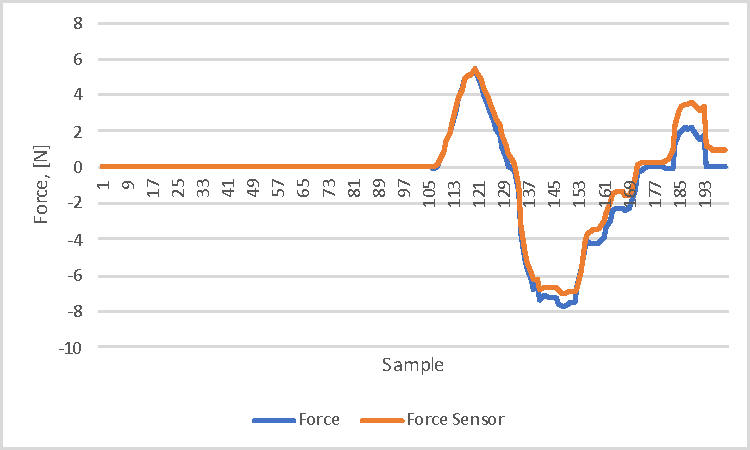
\includegraphics[width=80mm]{fig/results/syst_error.pdf}
	\end{center}
	\vspace{-4mm}
	\caption[Actual and Measured Forces in X-direction]
	{Actual and Measured Forces in X-direction}
	\label{fig:Syst_err}
	\vspace{-2mm}
\end{figure}

However, disadvantages would be addition of the cost to already expensive system and possible biocompaitibily and sterilization issues. Also addition of the weight to the arm could alter robot performance, however, since the device will be placed close to the center of rotation of the robot arm, it will have minimal affect on the moment of inertia  in comparison to sensors added to the grippers.

Z Device and X-Y device do not work together at the same time, because created X-Y device takes the Z-component of the force and slightly restricts rotation of the shaft. In order to solve that issue, we can change mechanical design of the X-Y device by increasing the size of the sleeve and adding slippery material between the shaft and the sleeve (Figure \ref{fig:NewXYDesign}). However, it will cause other issues with increased incision size to 1.9 cm. Usually size of the incision should be in range 1-2 cm. It will be still in appropriate range, however the recovery time would increase. Another option could be moving the X-Y device on the top of cannula or changing the cannula design and implementing sensor right on the cannula.

\begin{figure}[h]
	\begin{center}
		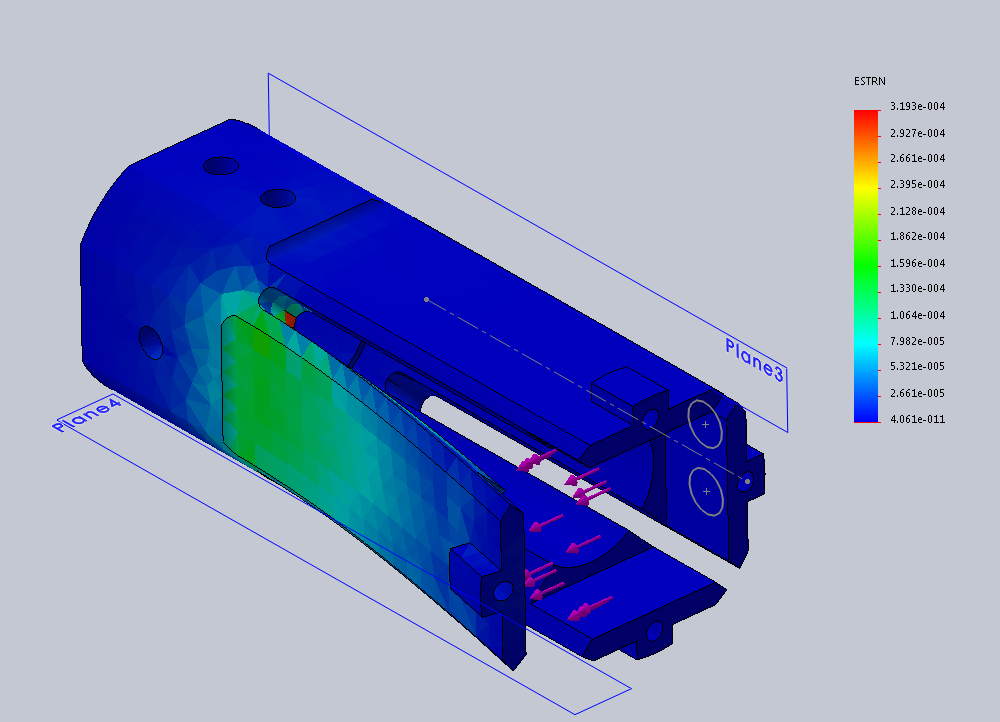
\includegraphics[width=120mm]{fig/methods/NEW_SLEEVE_STRAIN.png}
	\end{center}
	\vspace{-4mm}
	\caption[New X-Y Device Design]
	{New X-Y Device Design}
	\label{fig:NewXYDesign}
	\vspace{-2mm}
\end{figure}

Another thing that could be changed is type of sensor. Use of QTC-pills seem to be promising approach, since it has smaller size and higher sensitivity. However, it has nonlinear output, meaning some electrical design and calibration complications.

Some of the requirements for the devices were met, such as sensitivity, resolution, force measurement range, signal-to-noise ratio. However, the system has some major drawbacks due to high hysteresis and errors.

The created sensor gives 3-DOF force feedback. Showing that it is possible to add force-feedback in the daVInci robot without major changes of the existing system. However, not all of the requirements for the force measuring system were satisfied, meaning that the sensors need further improvements in both electrical and mechanical designs.